\chapter{Odometry}

\section*{Wheel odometry}
We are currently able to receive odometry data from the wheels, but only at low speeds. The issue we encountered with the AX-12W motors is that they return invalid position values in the range between 330º and 350º. To work around this, we switched to using the Present Speed register instead. However, this approach requires the robot to operate at relatively low speeds to maintain accuracy.

\section*{Odometry Validation}
To ensure our odometry is accurate enough for use in SLAM, it must first be validated. Without accurate odometry, the SLAM-generated map may not align correctly with the real-world environment. One of the most effective ways to validate odometry is by using an overhead camera. This camera can track the robot’s movement in real-time and provide a ground-truth odometry reference. We will compare the camera-derived odometry with both wheel odometry and LiDAR-based odometry separately. By analyzing the deviations, we can determine which method is more accurate. If neither source is sufficiently reliable on its own, we will fuse the data from both using an Extended Kalman Filter (EKF) to improve overall accuracy.
\newline

Initially, we considered two approaches for tracking the movement of robots. The first method involved using colored markers placed on the robots and tracking their motion using OpenCV. However, this approach has limitations, as color detection can be unreliable due to lighting variations and camera inaccuracies. The second method we explored was using the ArUco library, which generates unique, square-shaped markers similar to QR codes (Figure \ref{fig:aruco-marker}). These markers can be attached to the robots and tracked using computer vision techniques. This method offers higher accuracy and robustness compared to color-based tracking, as ArUco markers are designed for reliable detection even under varying conditions.

\begin{figure}[H]
    \centering
    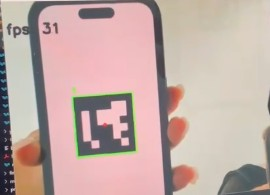
\includegraphics[width=0.3\linewidth]{assets/images/odometry/aruco.jpg}
    \caption{ARUCO 6X6 marker ID: 1}
    \label{fig:aruco-marker}
\end{figure}

The experiment setting of the validation is done by placing the camera over the robot arena, such that the frame of the camera fits perfectly with the arena. This allows us to estimate the actual measurement by calculating from the size of the arena, which is known prior. The method then starts by tracking the position,$(x, y, \theta)$  , of the marker in the camera frame, and then we relate it to the internal representation map (Figure \ref{fig:aruco-tracker}). 

\begin{figure}[H]
    \centering
    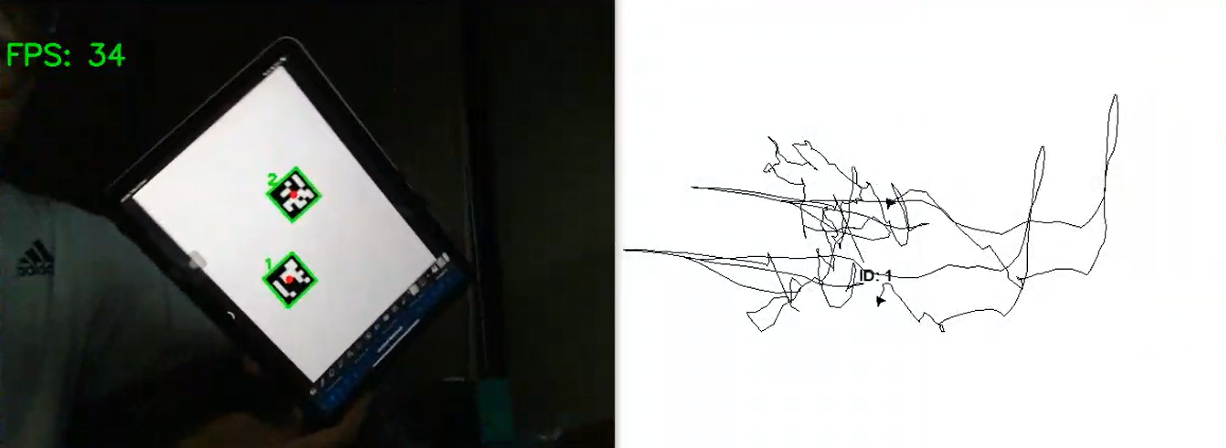
\includegraphics[width=0.9\linewidth]{assets/images/odometry/arcuo_tracker.png}
    \caption{ARUCO tracker using turtle}
    \label{fig:aruco-tracker}
\end{figure}

After that, we can calculate the error on the basis of many factors and methods. One way we would like to propose is the root mean square error of the trajectory over time, where the Euclidean distance and angular error between the ideal robot position commanded from the server and the actual robot position on the map.

\[
RMSE = \sqrt{\frac{1}{N} \sum_{i=1}^{N} (d_i^2 + w_{\theta} \theta_{\text{error}, i}^2)}, \quad \text{where } w_{\theta} \text{ is the weight of angle error, and}
\]
\[
\begin{array}{c c}
d_i = \sqrt{(x_{\text{actual}} - x_{\text{ideal}})^2 + (y_{\text{actual}} - y_{\text{ideal}})^2} & 
\theta_{\text{error}} = \theta_{\text{actual}} - \theta_{\text{ideal}}
\end{array}
\]


